\subsection{Summe \& Produkt}
Summe: stilisiertes großes Sigma
$$\sum\limits_{i = n}^n f(i) = \left \lbrace \begin{array}{ll}
                                                 f(m) + f(m + 1) + \dots + f(n) & \textrm{falls } n \geq m \\
                                                 0                              & \textrm{sonst}           \\
\end{array} \right.$$
Summe aller Elemente $i$ in einer Menge $I$
$$\sum\limits_{i \in I}$$
Produkt: stilisiertes großes pi
$$\prod\limits_{i=m}^{n} f(i) = \left \lbrace \begin{array}{ll}
                                                  f(m) \cdot f(m + 1) \cdot \dots \cdot f(n) & \textrm{falls } n \geq m \\
                                                  1                                          & \textrm{sonst}           \\
\end{array} \right.$$
Produkt aller Elemente $i$ in einer Menge $I$
$$\prod\limits_{i \in I}$$
\begin{itemize}
    \item[$i$] Laufvaribale / Indexvaribale, kann umbenannt werden, vorausgesetzt die neue Bezeichnung kommt noch nicht vor.
    \item[] $$\sum\limits_{i = m}^n f(i) = \sum\limits_{j = m}^n f(j)$$
    $$\prod\limits_{i = m}^n f(i) = \prod\limits_{j = m}^n f(j)$$
    \item[$m$] Laufanfang
    \item[$n$] Laufende
    \item $i;m;n \in \mathbb{Z}$
    \item Indexverschiebeung: Laufbeginn und ende können modifiziert werden.
    $$\sum\limits_{i=m}^n f(i) = \sum\limits_{i=m+k}^{n+k} f(i-k)$$
    $$\prod\limits_{i=m}^n f(i) = \prod\limits_{i=m+k}^{n+k} f(i-k)$$
    \begin{alignat*}{1}
        1+3+4+\dots+(2n-3)+(2n-1) & = \sum\limits_{i = 1}^n (2i-1)             \\
        & = \sum\limits_{i = 3}^{n + 2} (2(i - 2)-1) \\
        & = \sum\limits_{i = 0}^{n - 1} (2(i + 1)-1) \\
    \end{alignat*}
    \item Auseinandernehmen:
    $$\sum\limits_{i=m}^n (f(i) + g(i)) = \sum\limits_{i=m}^n (f(i)) + \sum\limits_{i=m}^n (g(i))$$
    \item Ausklammern
    $$\sum\limits_{i=m}^n (a \cdot f(i)) = a \sum\limits_{i=m}^n f(i)$$
    Beispiele:
    $$\sum\limits_{i=1}^n (2i-1) = \sum\limits_{i=1}^n (2i) - \sum\limits_{i=1}^n (1) = 2\sum\limits_{i=1}^n (i) - n$$
    $$\sum\limits_{i=1}^{100} (3i-4) = 3\sum\limits_{i=1}^{100} (i) - 400$$
    \item Doppelsummen
    $$\sum\limits_{i=m}^n \sum\limits_{j=a}^b f(i; j) = \sum\limits_{j=a}^b \sum\limits_{i=m}^n f(i; j)$$
\end{itemize}
\subsection{Vereinigung \& Schnitt}
$$\bigcup\limits_{i=m}^n A(i) = \left\lbrace \begin{array}{ll}
                                                 A(m) \cup A(m + 1) \cup + \dots + \cup A(n) & \textrm{falls } m \leq n \\
                                                 \emptyset                                   & \textrm{sonst}           \\
\end{array}  \right.$$
$$\bigcap\limits_{i=m}^n A(i) = \left\lbrace \begin{array}{ll}
                                                 A(m) \cap A(m + 1) \cap + \dots + \cap A(n) & \textrm{falls } m \leq n \\
                                                 \mathbb{M}                                  & \textrm{sonst}           \\
\end{array}  \right.$$
\subsection{Potenzgestze}
\begin{itemize}
    \item $x \in \mathbb{R};\ x^0 = 1$ auch $0^0=1$
    \item $x \in \mathbb{R};\ n \in \mathbb{N}^+;\ x^n = x \cdot x \cdot x \cdot x \dots \cdot x$ n mal
    \item $x \in \mathbb{R};\ x \not = 0;\ n = -1;\ x^{-1} \coloneqq \frac{1}{x}$ $0^{-1}$ nicht definiert
    \item $x \in \mathbb{R};\ a \not = 0;\ n = -m;\ m \in \mathbb{N}^+;\ x^{-m} = \frac{1}{x^{m}} = (x^{-1})^m$
    \item $x \in \mathbb{R};\ x \geq 0;\ m \in \mathbb{N}^+;\ x^{\frac{1}{m}} \coloneqq \sqrt[m]{x}$
    \item $x \in\mathbb{R};\ x > 0;\ m \in \mathbb{N}^+;\ x^{-\frac{1}{m}} \coloneqq (x^{-1})^{\frac{1}{m}}= (\frac{1}{x})^{\frac{1}{m}}=\sqrt[m]{\frac{1}{x}} = \frac{1}{\sqrt[m]{x}}$
    \item $x \in\mathbb{R};\ x \geq 0;\ m;n \in \mathbb{N}^+;\ x^{\frac{n}{m}} \coloneqq \left(\sqrt[m]{x}\right)^n = \sqrt[m]{x^n}$
    \item $x \in \mathbb{R};\ x > 0;\ m;n \in \mathbb{N}^+;\ m^{-\frac{n}{m}} \coloneqq \frac{1}{x^{\frac{n}{m}}} = \sqrt[m]{\frac{1}{x^n}} = \left(\frac{1}{\sqrt[m]{x}}\right)^n$
    \item $x \in \mathbb{R};\ x > 0;\ (x \geq 0 \textrm{ falls } \alpha > 0);\ \alpha \in \mathbb{R};\ x^\alpha$ als Grenzwert $x^{\alpha_k} = \lim\limits_{k \to \infty}\alpha_k = \alpha;\ \alpha \in \mathbb{Q}$
    $$\exp(z) = e^z = \sum\limits_{i = 0}^\infty \frac{z^i}{i!}$$
\end{itemize}
Voraussetzung : $x \in \mathbb{R};\ x > 0;\ \alpha; \beta \in \mathbb{R}$
\begin{alignat*}{1}
    x^{\alpha + \beta}            & = x^\alpha \cdot x^\beta                                                                                                        \\
    x^{\alpha \cdot \beta}        & = \left(x^\alpha\right)^\beta = \left(x^\beta\right)	\alpha                                                                     \\
    x^{-\alpha}                   & = \frac{1}{x^{\alpha}}                                                                                                          \\
    x^0                           & = 1;\ x^1 = x;\ x^{-1}    = \frac{1}{x}                                                                                         \\
    \left(x \cdot y\right)^\alpha & = x^\alpha \cdot y^\beta                                                                                                        \\
    x^{y^z}                       & = x^{\left(y^z\right)}                                                                                                          \\
    \textrm{Wurzel}               & = \sqrt[m]{x}                                                                                                                   \\
    \sqrt[m]{x}                   & = x^{\frac{1}{m}}                                                                                                               \\
    \sqrt[m]{\sqrt[n]{x}}         & = \left(x^{\frac{1}{n}}\right)^\frac{1}{m} = x^{\frac{1}{m \cdot n}=\sqrt[m \cdot n]{x}}                                        \\
    \sqrt[m]{x^n}                 & = \left(\sqrt[m]{x}\right)^n = x^{\frac{n}{m}}                                                                                  \\
    \sqrt[1]{x}                   & = x                                                                                                                             \\
    \sqrt[m]{x} \cdot \sqrt[n]{x} & = x^{\frac{1}{m}} \cdot x^{\frac{1}{n}} = x^{\frac{1}{n}+\frac{1}{m}} = x^{\frac{m+n}{m \cdot n}} = \sqrt[m \cdot n]{x^{m + n}}
\end{alignat*}
\subsection{Fakultäten}
\begin{itemize}
    \item Fakultät $0! \coloneqq 1;\ (n+1)!=n!(n+1)$ wächst sehr schnell.
    $$(n \geq 1)\ n! = \prod\limits_{i=1}^n i$$
    \item Kombinatorische Bedeutung: Anzahl der Anordnungen von $n$ Gegenständen in einer Reihe.
    \item Näherung durch Stirling-Formel:
    $$n! \approx \sqrt{2 \pi n} \left(\frac{n}{e}\right)^n$$
    \item Nährung durch Bill Gosper
    $$n! \approx \sqrt{2 \pi n + \frac{\pi}{3}}\left(\frac{n}{e}\right)^n$$
\end{itemize}
\subsection{Binominialkoeffizient}
$n \in \mathbb{N}; m \in \mathbb{N};\ \binom{n}{k}$  gelesen ''n über m'' $n < m \Rightarrow \binom{n}{m} = 0$ $n \geq m \Rightarrow \binom{n}{0} = 1,\ \binom{n}{1} = n,\ \binom{n}{n}$
$$\binom{n}{m} = \frac{n(n-1) \dots \cdot (n-m-1)}{1\cdot 2\cdot3 \dots m} = \frac{n!}{m!(n-m)!}$$
$$\binom{n}{m}=\binom{n}{n-m}$$ Jeweils $m$ viele Faktoren, da sich der Rest wegkürzt.
z.b:
$$\binom{4}{2} = \frac{4 \cdot 3 \cdot \cancel{2 \cdot 1}}{2 \cdot 1 \cdot \cancel{2 \cdot 1}} = \frac{12}{2} = 6;\ \binom{5}{3} = \binom{5}{2} = \frac{5 \cdot 4 \cdot  \cancel{3 \cdot 2 \cdot 1}}{2 \cdot 1 \cdot \cancel{3 \cdot 2 \cdot 1}} = 10$$
Kombinatorische Bedeutung: Anzahl der m-elementigen Teilmengen einer n-elementigen Menge
$$\binom{n}{m}+\binom{n}{m+1}=\binom{n+1}{m+1}$$
\begin{alignat*}{1}
    \binom{n}{m}+\binom{n}{m+1} & =\frac{n!}{m!(n-m)!}+\frac{n!}{(m+1)!(n-m-1)!}=\frac{n!(m+1)+n!(n-m)}{(m+1)!(n-m)!} \\
    & =\frac{(n+1)!}{(m+1)!((n+1)-(m+1))!}
\end{alignat*}
Pascalsches Dreieck: \\
\begin{tabularx}{\linewidth}{@{}*2{>{\centering\arraybackslash}X}}
    \begin{tikzpicture}
        \node (11) at (0, 0) {1};
        \node (21) at (-0.5, -0.5) {1};
        \node (22) at (0.5, -0.5) {1};
        \node (31) at (-1, -1) {1};
        \node (32) at (0, -1) {2};
        \node (33) at (1, -1) {1};
        \node (41) at (-1.5, -1.5) {1};
        \node (42) at (-0.5, -1.5) {3};
        \node (43) at (0.5, -1.5) {3};
        \node (44) at (1.5, -1.5) {1};
        \node (51) at (-2, -2) {1};
        \node (52) at (-1, -2) {4};
        \node (53) at (0, -2) {6};
        \node (54) at (1, -2) {4};
        \node (55) at (2, -2) {1};
        \node (61) at (-2.5, -2.5) {1};
        \node (62) at (-1.5, -2.5) {5};
        \node (63) at (-0.5, -2.5) {10};
        \node (64) at (0.5, -2.5) {10};
        \node (65) at (1.5, -2.5) {5};
        \node (66) at (2.5, -2.5) {1};
    \end{tikzpicture} &
    \begin{tikzpicture}
        \node (11) at (0, 0) {$\binom{0}{0}$};
        \node (21) at (-0.5, -0.5) {$\binom{1}{0}$};
        \node (22) at (0.5, -0.5) {$\binom{1}{1}$};
        \node (31) at (-1, -1) {$\binom{2}{0}$};
        \node (32) at (0, -1) {$\binom{2}{1}$};
        \node (33) at (1, -1) {$\binom{2}{2}$};
        \node (41) at (-1.5, -1.5) {$\binom{3}{0}$};
        \node (42) at (-0.5, -1.5) {$\binom{3}{1}$};
        \node (43) at (0.5, -1.5) {$\binom{3}{2}$};
        \node (44) at (1.5, -1.5) {$\binom{3}{3}$};
        \node (51) at (-2, -2) {$\binom{4}{0}$};
        \node (52) at (-1, -2) {$\binom{4}{1}$};
        \node (53) at (0, -2) {$\binom{4}{2}$};
        \node (54) at (1, -2) {$\binom{4}{3}$};
        \node (55) at (2, -2) {$\binom{4}{5}$};
        \node (61) at (-2.5, -2.5) {$\binom{5}{0}$};
        \node (62) at (-1.5, -2.5) {$\binom{5}{1}$};
        \node (63) at (-0.5, -2.5) {$\binom{5}{2}$};
        \node (64) at (0.5, -2.5) {$\binom{5}{3}$};
        \node (65) at (1.5, -2.5) {$\binom{5}{4}$};
        \node (66) at (2.5, -2.5) {$\binom{5}{5}$};
    \end{tikzpicture}
\end{tabularx}
$$\sum\limits_{k=1}^n \binom{k}{m} = \binom{1}{m}+\binom{2}{m}+ \dots + \binom{m}{n}+\binom{m}{m}+\binom{m+1}{m}+\dots+\binom{n}{m}=\binom{n+1}{m+1}$$
$$\sum\limits_{k=1}^n\binom{k}{1} = \frac{n(n+1)}{2}$$
Binomialsatz
$$(a+n)^n=\sum\limits_{m=0}^n\binom{n}{m}a^{n-m}b^m=a^n+\binom{n}{1}a^{n-1}b+\binom{n}{2}a^{n-2}b^2+\dots + \binom{n}{n-1}ab^{n-1}+b^n$$
\subsection{Umformungen von Termen}
Erklärung: Ein (Funktions)Term ist ein ''vernünftig'' aufgebauter Ausdruck zur Berechnung einer Funktion.

Terme könne aus folgendem bestehen
\begin{itemize}
    \item Zeichen für Variablen und Parameter $x;\ y;\ z;\ a;\ b$
    \item Zahlen, Konstanten
    \item Operationen
    \item Funktionszeichen $\exp;\ \sin;\ cos;\ $
    \item technische Zeichen $(;);\lbrace;\rbrace,\lbrack,\rbrack$
\end{itemize}
Funktionsbezeichung: $f;\ f(x);\ f(x;y)$ Wir bezeichnunen Terme ähnlich wie Funktionen. Aber: Ein Term definiert eine Funktion aber nicht umgekehrt.


\underline{Ziel:} Möglichst einfache Terme für eine Funktion finden. Zu einem Term $f(x)$ gehört ein maximaler Definitionsbereich (auch natürlicher Definitionsberiech). Das ist die größte Teilmenge $D \in \mathbb{R}$ für die alle Teilterme von $f$ definiert sind. Dieser DB kann eventuell weiter eingeschränkt werden. Bezeichnungen für den Definitionsberiech: $D_f;\ \textrm{DBb}(f), D$


Beispiel: $f(x) = \frac{x^2-x-6}{x+2}\quad D_f=\mathbb{R}\setminus\lbrace-2\rbrace$
$$f(x)= \frac{(x-3)(x+2)}{x+2} = x-3\quad | x \not = -2$$

\subsubsection{Faktorisieren}
\begin{description}
    \item[Binomische Formeln] \
    \begin{itemize}
        \item[1.] $(a+b)^2=a^2+2ab+b^2$
        \item[2.] $(a-b)^2=a^2-2ab+b^2$
        \item[3.] $(a-b)(a+b)=a^2-b^2$
    \end{itemize}
    \item[Summenformel] \
    \begin{itemize}
        \item $(1-x)(1+x+x^2+\dots +x^n)=1-x^{n+1}$
        \item $(x-1)(1+x+x^2+\dots +x^n)=x^{n+1}-1$
    \end{itemize}
    \item[Distributivgesetze] \
    \begin{itemize}
        \item $a(a+b)=ab+ac$
        \item $(a+b)(c+d) = ac +ad + bc +bd$
    \end{itemize}
    \item[Vieta] $(x-a)(x-b) = x^2 - (a+b)x+ab$
    \item[Wurzel aus Nenner] $\frac{1}{\sqrt{2}}=\frac{\sqrt{2}}{2}$
    $$\frac{2+\sqrt{3}}{2-\sqrt{3}}=\frac{2+\sqrt{3}}{2-\sqrt{3}} \cdot \frac{2+\sqrt{3}}{2+\sqrt{3}}=\frac{4+4\sqrt{3}+3}{4-3}=7+4\sqrt{3}$$
\end{description}
\subsection{Proportionalität}
Größe
\begin{itemize}
    \item Bezeichnung $X$, z.B. Fahrstrecke
    \item zugehörige Wertemenge, hier stehts $X\in \mathbb{R}$ (notfalls runden mit Verstand)
    \item eventuell mit Einheit, schreibweise $x \in X$
    \item Zwei Größen $x;\ Y$ i.a. nicht unabhänig.
    \item $E \subseteq X \times Y$
    \item $X$ und $Y$ heißen proportional, $X \sim Y$, wenn $(\exists c)\ (x;y) \in E \Leftrightarrow \frac{x}{y}=c$ z.B. Farstrecke $\sim$ Benzinverbrauch
    \item $X$ und $Y$ heißen umgekehrt proportional, $x \sim \frac{1}{Y}$, wenn $(\exists c)\ (x;y) \in E \Leftrightarrow x \cdot y = c$. Z.B.: Arbeiteranzahl $\sim \frac{1}{\textrm{Arbeitszeit}}$
    \item $X \sim Y;\ (x_1;y_1);\ (x_2;y_2) \in E \Rightarrow \frac{x_1}{y_1} = c = \frac{x_2}{y_2}$
    \item $X \sim \frac{1}{Y};\ (x_1;y_1);\ (x_2;y_2) \in E \Rightarrow x_1 \cdot y_1 = c = x_2 \cdot y_2$
    \item mehr als zwei Größen: Für die Zerlegung von 7,2t brauchen 14 Arbeiter 8h. Wie viele Arbeiter braucht man, um 6t in 8 h zu zerlgen. \\
    Propotionalitätsbeziehung zwichen $$E \subseteq X \times  Y \times Z\ : (x; y; z) \in E$$ $$(\exists i_x; i_y; i_z \in \lbrace -1; 1 \rbrace) (\exists c)\ (x;y;z) \in E \Leftrightarrow x^{i_x}y^{i_y}z^{i_z} = c$$
    $$A \sim S;\ A \sim \frac{1}{T}$$
    $$\frac{14z \cdot 8h}{7{,}2t}=c=\frac{a \cdot 8h}{6t} \Rightarrow a = \frac{6t}{7{,}2t}\cdot \frac{8h}{8h} \cdot 14z \approx 12z$$
\end{itemize}
\subsubsection{Prozentrechnung}
\begin{itemize}
    \item Spezialfall der Proportionalität
    \item Zwei größen:\
    \begin{itemize}
        \item Prozente
        \item andere Größe
    \end{itemize}
    \item $1\% = \frac{1}{100}$
    \item $1\permil = \frac{1}{1000}$
    \item Grundwert $G \hat{=} 100\%$, Prozentwert $W \hat{=} p\%$
    $$\frac{G}{100\%} = \frac{W}{p\%}$$
\end{itemize}
\subsection{Gleichungen}
$$f(x)=g(x)$$
\begin{description}
    \item[Lösungsmenge] $\mathbb{L} = \lbrace x \in D_f \cap D_g | f(x) = g(x) \rbrace$ explizit angeben.
    \item[Äquivalenete Umformung] ändert $\mathbb{L}$ nicht. Zwei gleichungen heißen äquivalent wenn ihre Lö-sungsmengen gleich sind.
    $$f(x)= g(x) \Leftrightarrow \widetilde{f}(x) = \widetilde{g}(x)$$
    \item[nichtäquivalente Umformungen]
    Folgerungen $f(x) = g(x) \Rightarrow \widetilde{f}(x) = \widetilde{g}(x)$, d.h. $\mathbb{L} \subseteq \widetilde{\mathbb{L}}$ Probe!
    \begin{alignat*}{2}
        x-2     & = 3 \quad    &  & \mathbb{L} = \lbrace 5 \rbrace     \\
        (x-2)^2 & = 3^2  \quad &  & \mathbb{L} = \lbrace -1; 5 \rbrace \\
    \end{alignat*}
    \item[spezielle Umformungen] $t(x)$ sei ein weiterer Term mit $D_f \cap D_g \subseteq D_f$
    \begin{alignat*}{2}
        f(x) = g(x) & \Leftrightarrow f(x) + t(x)       &  & = g(x) + t(x)                                     \\
        f(x) = g(x) & \Leftrightarrow f(x) \cdot t(x)   &  & = g(x) \cdot t(x)\textrm{ falls } t(x) \not = 0   \\
        f(x) = g(x) & \Leftrightarrow \frac{f(x)}{t(x)} &  & = \frac{g(x)}{t(x)}\textrm{ falls } t(x) \not = 0 \\
    \end{alignat*}
    $h : D_h \longrightarrow \mathbb{R}$ Funktion, , $f\lbrack D_f \cap D_g \rbrack \cup g\lbrack D_f \cap D_g \rbrack \subseteq D_h$
    $$f(x) = g(x) \Rightarrow h(f(x)) = h(g(x))$$
    Ist $h$ insbesondere umkehrbar (injektiv), dann gilt
    $$f(x) = g(x) \Leftrightarrow h(f(x)) = h(g(x))$$
    \item[Lineare Gleichungen] $ax + b = 0 \quad a \not = 0$
    \begin{alignat*}{2}
        & \Leftrightarrow ax &  & = -b           \\
        & \Leftrightarrow x  &  & = \frac{-b}{a} \\
    \end{alignat*}
    \begin{alignat*}{3}
        & \quad \frac{7x+91}{17x+221} &  & = 11                 &  & | \cdot (17x + 221) \\
        & \Leftrightarrow 7x + 91     &  & = 11 \cdot (17x+221)                          \\
        & \Leftrightarrow 7x + 91     &  & = 187x + 2431                                 \\
        & \Leftrightarrow 0           &  & = 180x +2340         &  & |-2340              \\
        & \Leftrightarrow 180x        &  & = -2340              &  & | :180              \\
        & \Leftrightarrow x           &  & = -13                                         \\
    \end{alignat*}
    $$\mathbb{D} = 17x+221 \not = 0$$
    $$x \not \in \mathbb{D}$$
    \item[Gleichung mit Beträgen] $|a| = \sqrt{a^2}$
    $$\begin{array}{ll}
          |a| \geq 0                  & |a| = 0 \Leftrightarrow a = 0              \\
          |a \cdot b| = |a| \cdot |b| & \frac{|a|}{|b|} = \left|\frac{a}{b}\right| \\
          |a+b| \leq  |a| + |b|       & ||a|-|b|| \leq |a-b|                       \\
    \end{array}$$
    \begin{itemize}
        \item $|f(x)| = c$ \
        \begin{itemize}
            \item falls $c<0$, so $\mathbb{L}= \emptyset$
            \item falls $c\geq0$: $|f(x)| = c \Leftrightarrow f(x) = c \vee f(x) = -c;\ \mathbb{L} = \mathbb{L}_1 \cup \mathbb{L}_2$
        \end{itemize}
        \item $|f(x)| = |g(x)| \Leftrightarrow f(x)^2 = g(x)^2$
        \item $|f(x)| = |g(x)| \Leftrightarrow \left|\frac{f(x)}{g(x)}\right| = 1 \Leftrightarrow \frac{f(x)}{g(x)} = 1 \vee \frac{f(x)}{g(x)} = -1$
        \item[Allgemein:] Vollständige Fallunterschiedung
        $$|x-1|+|x+1|=10$$
        \begin{itemize}
            \item[Fall 1] $x-1 \geq 0;\ x+1 \geq 0 \ \Leftrightarrow x \geq 1;\ x\geq -1 \Leftrightarrow x>1$
            \begin{alignat*} {1}
            (x-1) + (x+1) & = 10                \\
            2x            & = 10                \\
            x             & = 5                 \\
            \mathbb{L}_1  & = \lbrace 5 \rbrace \\
            \end{alignat*}
            \item[Fall 2] $x-1 \geq 0;\ x+1 < 0 \ \Leftrightarrow x \geq 1;\ x < -1 \quad \mathbb{L}_2 = \emptyset$
            \item[Fall 3] $x-1 < 0;\ x+1 \geq 0 \ \Leftrightarrow x < 1;\ x\geq -1 \Leftrightarrow -1 \leq x < 1$
            \begin{alignat*} {1}
                -(x-1) + (x+1) & = 10        \\
                2              & = 10        \\
                \mathbb{L}_3   & = \emptyset \\
            \end{alignat*}
            \item[Fall 4] $x-1 < 0;\ x+1 < 0 \ \Leftrightarrow x < 1;\ x < -1 \Leftrightarrow x<-1$
            \begin{alignat*} {1}
                -(x-1) +(-(x+1)) & = 10                 \\
                -2x              & = 10                 \\
                x                & = -5                 \\
                \mathbb{L}_1     & = \lbrace -5 \rbrace \\
            \end{alignat*}
            \item[$\mathbb{L}$] = $\mathbb{L}_1 \cup \mathbb{L}_2 \cup \mathbb{L}_3 \cup \mathbb{L}_4 = \lbrace -5; 5\rbrace$
        \end{itemize}
    \end{itemize}
    \item[Quadratische Funktionen]
\end{description}
